\section{Aufgabe 21}
\subsection{a)-c)}
siehe Anhang.

\subsection{d)}
Siehe Python-Datei.

\begin{align*}
  W = \begin{pmatrix}
      -0,58 &  1,42 \\
      1,83  &  -0,56 \\
      \end{pmatrix}
\end{align*}

\begin{align*}
  b = \begin{pmatrix}
      -0,48 \\
      0,61 \\
      \end{pmatrix}
\end{align*}

\subsection{e)}
Mit

\begin{align}
  \begin{pmatrix}
    W_{11} & W_{12} \\
    W_{21} & W_{22} \\
  \end{pmatrix}
  \cdot
  \begin{pmatrix}
    x \\
    y \\
  \end{pmatrix}
   +
  \begin{pmatrix}
    b_1 \\
    b_2 \\
  \end{pmatrix}
   =
  \begin{pmatrix}
    f_1 \\
    f_2 \\
  \end{pmatrix}
\end{align}

und $f_1 =f_2$ folgt

\begin{align*}
  & W_{11}x + W_{12}y +b_1 = W_{21}x+ W_{22}y+b_2 \\
  => & y(x)=\frac{b_2-b_1+ x \cdot (W_{21}-W_{11})}{W_{12}-W_{22}} \\
\end{align*}

In Abbildung \ref{abb:1} sind die zwei Populationen dargestellt und die oben
berechnete Trennung der beiden Populationen.
$f_1 = f_2$ kann angenommen werden, da die Punkte auf der Geraden keiner Population
zugeordnet werden können, da sie weder unter noch über der Geraden liegen, deshalb
müssen $f_1$ und $f_2$ gleich sein.
\begin{figure}
  \centering
  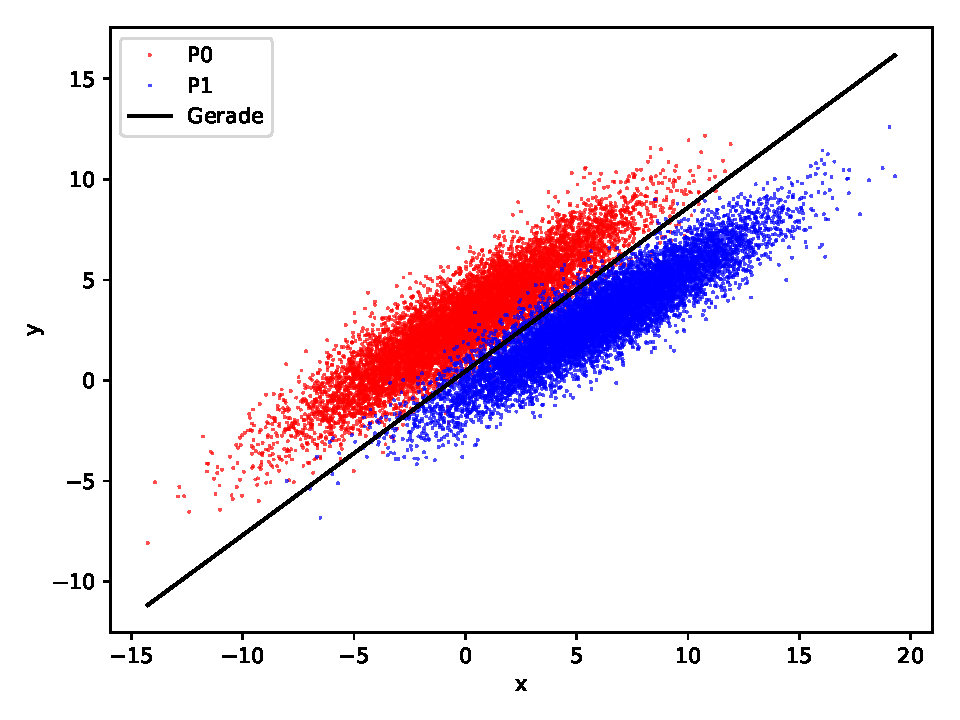
\includegraphics[scale=0.9]{Aufgabe21/Plot.pdf}
  \caption{Populationen mit der berechneten Trennung.}
  \label{abb:1}
\end{figure}

\begin{figure}
  \centering
  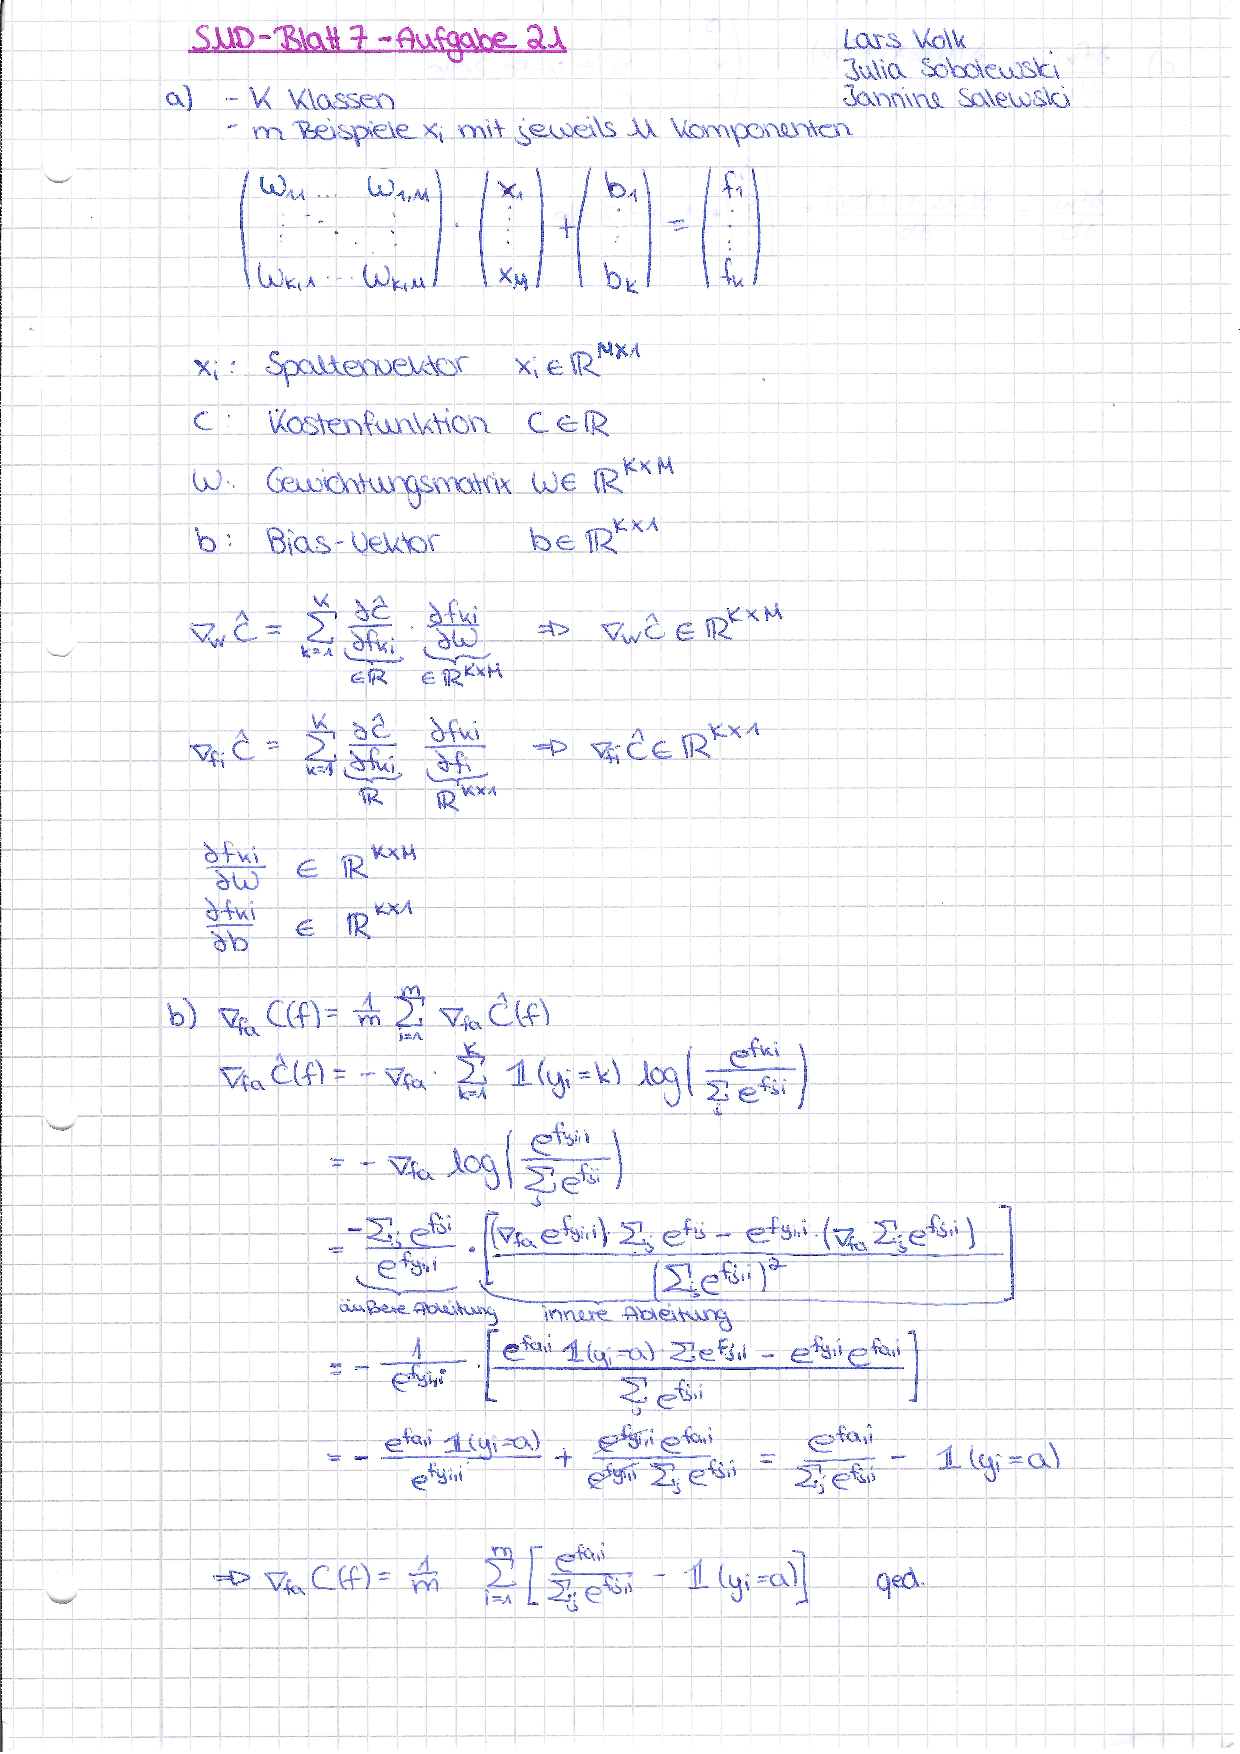
\includegraphics[scale=0.8]{Aufgabe21/page-1.pdf}
\end{figure}
\begin{figure}
  \centering
  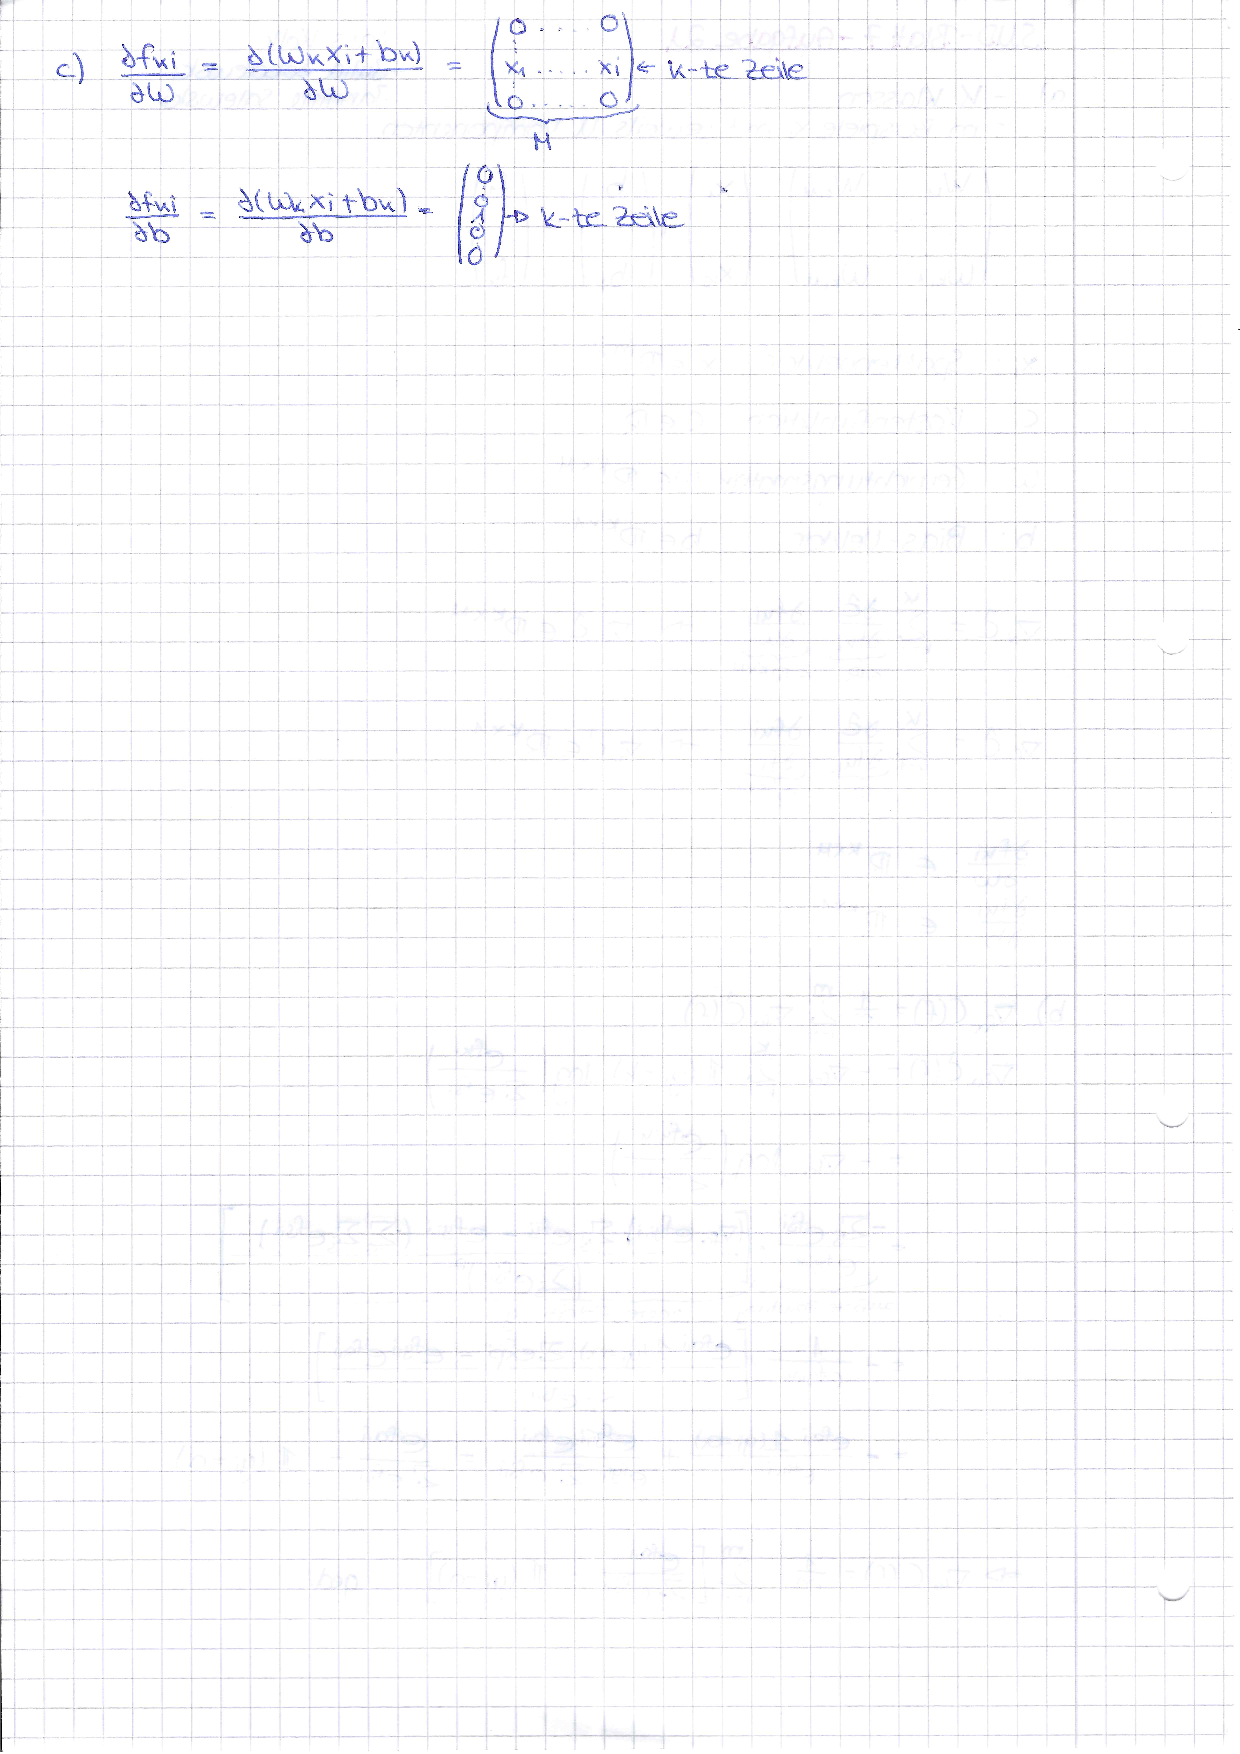
\includegraphics[scale=0.8]{Aufgabe21/page-2.pdf}
\end{figure}
